\documentclass[11pt,a4paper]{article}

\usepackage[spanish,es-noshorthands]{babel}
\usepackage[T1]{fontenc}
\usepackage[utf8]{inputenc}
\usepackage{lmodern}
\usepackage[a4paper,margin=2.4cm]{geometry}
\usepackage{amsmath}
\usepackage{booktabs}
\usepackage{array}
\usepackage{tabularx}
\usepackage{graphicx}
\usepackage{float}
\usepackage{caption}
\usepackage{enumitem}
\usepackage{xcolor}
\usepackage{hyperref}
\usepackage{xurl}
\usepackage{natbib}

\hypersetup{
    colorlinks=true,
    linkcolor=blue!60!black,
    citecolor=blue!60!black,
    urlcolor=blue!60!black,
    pdftitle={Guia sencilla para explicar el proyecto TD3 de protesis mioelectrica},
    pdfauthor={Proyecto EMG Prosthesis TD3}
}

\newcolumntype{L}[1]{>{\raggedright\arraybackslash}p{#1}}
\newcolumntype{Y}{>{\raggedright\arraybackslash}X}

\title{\textbf{Guia Sencilla para Explicar el Proyecto}\\
\large Version de charla para publico con poca base tecnica}
\author{Proyecto \texttt{EMG\_Prosthesis\_TD3}}
\date{26 de marzo de 2026}

\begin{document}
\maketitle

\begin{abstract}
Esta guia sirve para explicar el proyecto de forma sencilla. La idea central es muy simple: se quiso ensenar a una protesis mioelectrica a seguir la apertura de una mano de referencia sin moverse de forma brusca ni gastar accion de mas. El camino no fue lineal. Primero hubo que arreglar el problema y encontrar un benchmark valido; despues hubo que buscar una mejora real sin destruir el tracking. El punto final de la charla es el agente residual \texttt{Agent1850}, que mantiene casi el mismo tracking del benchmark \texttt{Agent7250} pero con menos esfuerzo y menos saturacion.
\end{abstract}

\tableofcontents
\newpage

\section{La idea general en una frase}

El proyecto intenta que una protesis aprenda a moverse de forma continua a partir de senales musculares y de estado, para copiar una referencia parecida al movimiento de una mano humana \citep{fuertes2026continuous,chen2023review}.

\section{Diccionario basico}

\begin{table}[H]
\centering
\caption{Palabras clave explicadas de forma simple}
\small
\begin{tabularx}{\linewidth}{@{}L{3.2cm}Y@{}}
\toprule
Termino & Explicacion sencilla \\
\midrule
EMG & Senal electrica de los musculos. Es una pista de lo que la persona quiere hacer. \\
Glove & Guante con sensores que da una referencia de movimiento. Aqui se usa como ``lo que la protesis deberia seguir''. \\
Protesis & La mano o sistema que queremos controlar. \\
TD3 & Un algoritmo de aprendizaje por refuerzo para acciones continuas \citep{fujimoto2018td3}. \\
Reward & La nota que recibe el agente. Si sigue bien la referencia y no se mueve de forma brusca, la nota mejora. \\
Tracking & Que tan bien la protesis sigue a la referencia. \\
Saturacion & Cuando la accion se pega demasiado al borde maximo o minimo del actuador. \\
Checkpoint & Una copia guardada del agente en cierto episodio para poder auditarlo o testearlo. \\
Residual policy & Una politica que no reemplaza a la anterior, sino que le suma una correccion pequena \citep{silver2018residual,schaff2020shared,resfit2025}. \\
Alpha residual & El tamano de esa correccion. Si es pequeno, corrige poco; si es grande, corrige mucho. \\
\bottomrule
\end{tabularx}
\end{table}

\section{Como se puede contar la historia del proyecto}

La historia se puede explicar en cuatro pasos:
\begin{enumerate}[leftmargin=1.5em]
\item habia una idea base correcta: usar TD3 para controlar una protesis de forma continua;
\item antes de comparar agentes hubo que arreglar la reward y el simulador;
\item el primer gran benchmark valido fue \texttt{Agent7250};
\item despues se abrio una fase nueva: mejorar ese benchmark sin perder tracking.
\end{enumerate}

\begin{figure}[H]
\centering
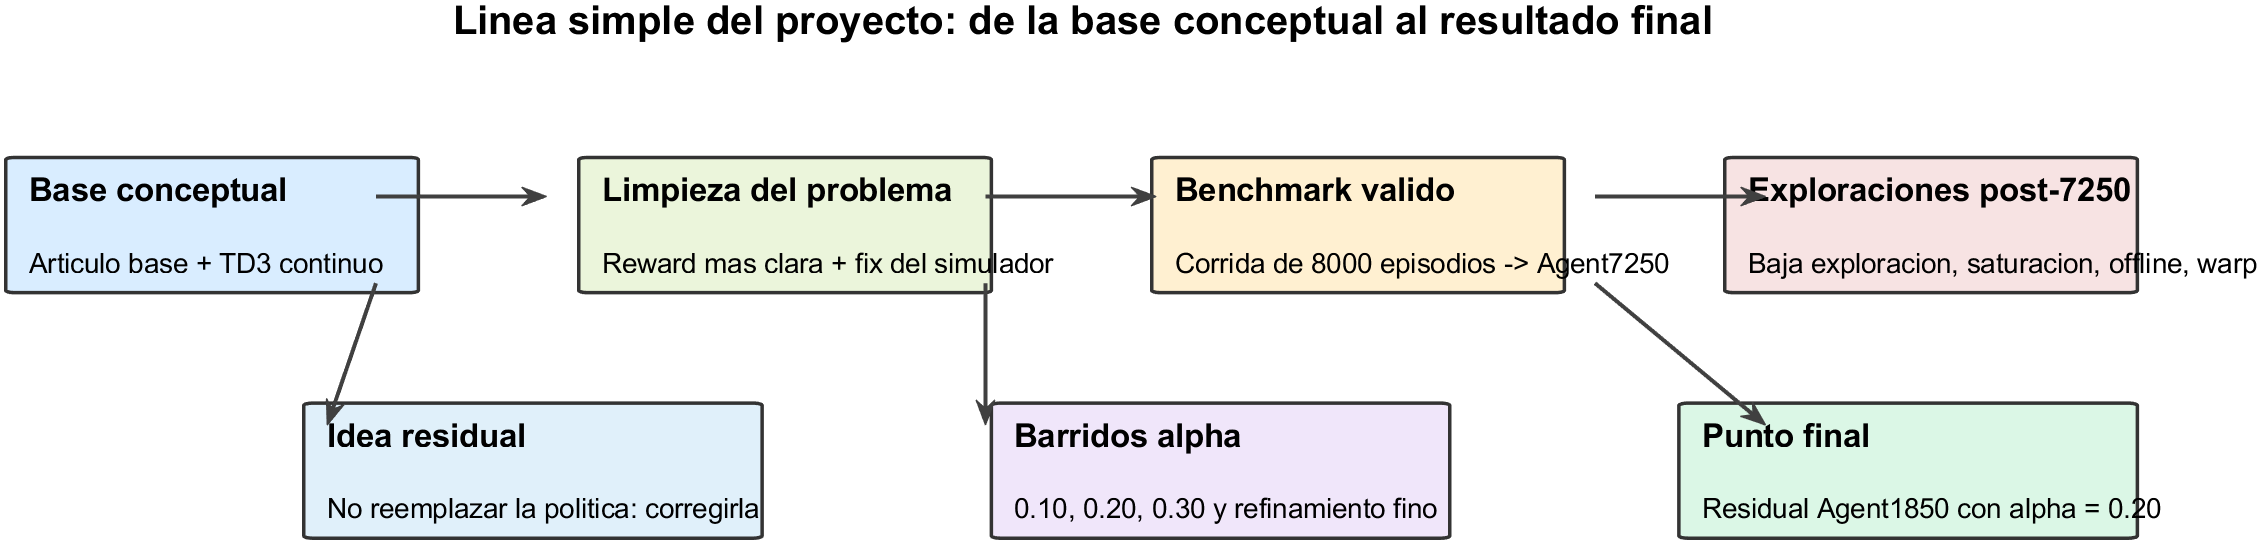
\includegraphics[width=0.96\linewidth]{figures/charla_linea_proyecto_20260326.png}
\caption{Linea simple del proyecto. Esta figura sirve para contar la historia sin entrar aun en detalles matematicos.}
\end{figure}

\paragraph{Como explicarla oralmente.}
Primero se dice que el proyecto no termino en la primera corrida buena. Al principio hubo que limpiar el problema. Luego aparecio \texttt{Agent7250} como benchmark serio. Despues se probaron varias ideas nuevas. La unica que realmente mejoro el compromiso global fue la politica residual.

\section{Que hacia el benchmark \texttt{Agent7250}}

El benchmark valido quedo con estas ideas:
\begin{itemize}[leftmargin=1.5em]
\item observacion \texttt{markov52};
\item reward \texttt{trackingMseActionRateReward};
\item TD3 feedforward;
\item accion cuantizada para respetar el actuador real.
\end{itemize}

Esto significa, en lenguaje simple, que el agente ve un estado resumido del sistema y aprende a escoger cuatro acciones continuas. Luego el entorno transforma esas acciones en comandos efectivos compatibles con la protesis.

\section{Por que no se cerro el proyecto con \texttt{Agent7250}}

\texttt{Agent7250} seguia bien la referencia, pero aun pagaba bastante en esfuerzo y saturacion. Por eso no bastaba con decir ``ya funciona''. La pregunta nueva fue:

\begin{quote}
\emph{Podemos conservar casi el mismo tracking, pero movernos de forma menos agresiva?}
\end{quote}

Ese cambio de pregunta es muy importante, porque explica por que hubo tantas pruebas despues del benchmark.

\section{Experimentos que se probaron despues}

\begin{table}[H]
\centering
\caption{Experimentos posteriores al benchmark y lectura simple}
\small
\begin{tabularx}{\linewidth}{@{}L{3.2cm}Y Y@{}}
\toprule
Idea & Por que parecia buena & Que paso al final \\
\midrule
Bajar exploracion & Menos ruido podia suavizar una politica ya buena & Suavizo, pero empeoro demasiado el tracking. \\
Exploracion cerca del umbral & El actuador tenia una discontinuidad real & No mejoro el mejor casi-acierto. \\
Reward de saturacion & Castigar el borde parecia razonable & La politica se volvio demasiado timida. \\
Warm-start offline & Darle un prior suave al agente nuevo & Tambien quedo demasiado conservador. \\
Warp de accion & Alinear mejor accion continua y actuador & La politica se volvio demasiado agresiva. \\
Residual TD3 & Corregir una politica buena en vez de rehacerla & Fue la primera mejora aceptable y defendible. \\
\bottomrule
\end{tabularx}
\end{table}

\section{La idea que si funciono: politica residual}

La idea residual se puede explicar con esta frase:

\begin{quote}
No tiremos la politica buena. Mantengamos a \texttt{Agent7250} y aprendamos solo una pequena correccion.
\end{quote}

La formula simple es:
\[
\text{accion final} = \text{accion base} + \alpha_{\mathrm{res}} \cdot \text{correccion}.
\]

\paragraph{Que significa eso en palabras.}
\begin{itemize}[leftmargin=1.5em]
\item la \textbf{accion base} es lo que ya hacia \texttt{Agent7250};
\item la \textbf{correccion} es un ajuste nuevo que aprende otra rama pequena;
\item \(\alpha_{\mathrm{res}}\) dice cuanto dejamos corregir.
\end{itemize}

\paragraph{Como explicar el alpha.}
\begin{itemize}[leftmargin=1.5em]
\item si \(\alpha\) es muy pequeno, la correccion casi no alcanza y todo queda demasiado parecido al benchmark;
\item si \(\alpha\) es muy grande, la correccion manda demasiado y se vuelve facil romper el equilibrio;
\item por eso se hicieron barridos de \(\alpha\): para encontrar un punto intermedio.
\end{itemize}

\section{Grafica de aprendizaje: como leerla}

\begin{figure}[H]
\centering
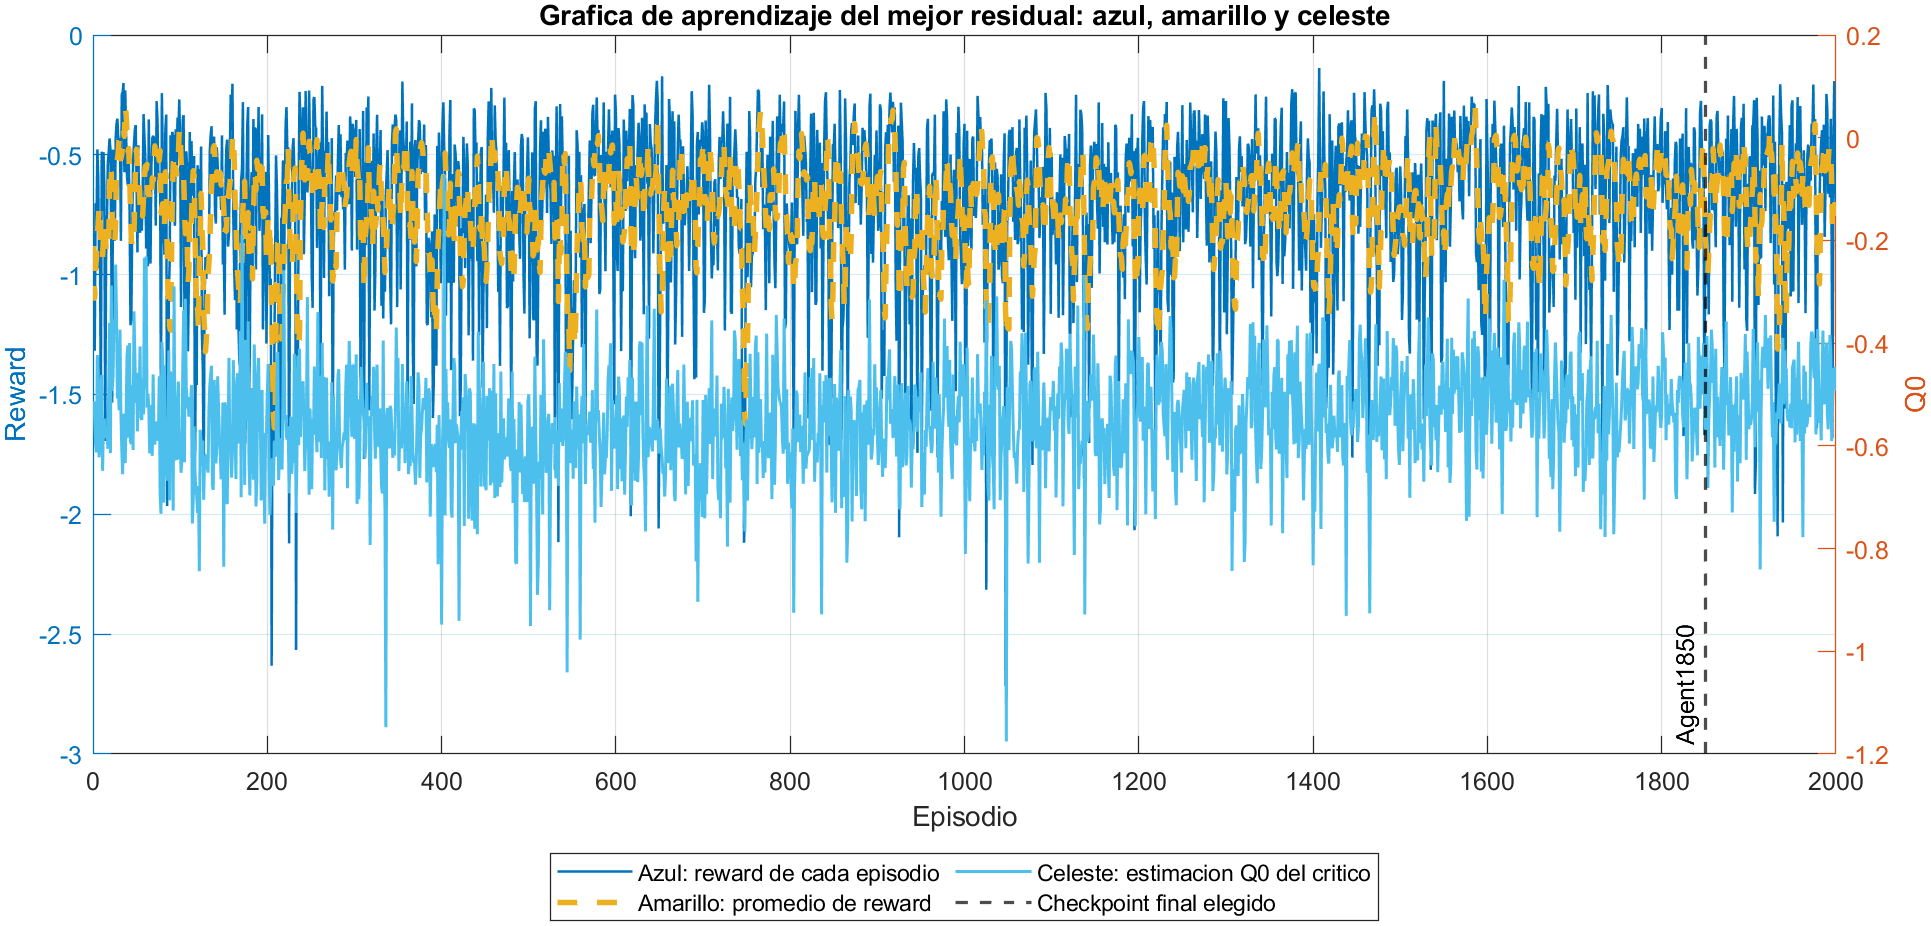
\includegraphics[width=0.96\linewidth]{figures/charla_training_residual_20260326.png}
\caption{Grafica didactica del entrenamiento residual. Esta es una de las figuras mas utiles para explicar el aprendizaje.}
\end{figure}

\paragraph{Linea azul.}
Es la reward de cada episodio. Sube y baja mucho porque cada episodio puede salir un poco distinto. No hay que juzgar el entrenamiento solo por esta linea.

\paragraph{Linea amarilla.}
Es el promedio de reward. Esta es la linea mas util para explicar la tendencia general. Si sube, el entrenamiento en promedio va mejorando. Si cae de forma sostenida, algo va mal.

\paragraph{Linea celeste.}
Es el \texttt{Q0}, una estimacion interna del critico. Para una charla sencilla basta decir que es ``la confianza del modelo sobre el valor esperado de sus decisiones''. Si cambia de forma razonable mientras mejora la linea amarilla, el aprendizaje parece coherente. Si se dispara o se hunde sin mejora real, puede haber desajuste.

\paragraph{Linea vertical negra.}
Marca el checkpoint elegido, \texttt{Agent1850}. Aqui es importante explicar algo clave del proyecto: el mejor agente no se eligio por intuicion ni por ``verse bonito'' en entrenamiento, sino por auditoria y test.

\section{Grafica de test: como leerla}

\begin{figure}[H]
\centering
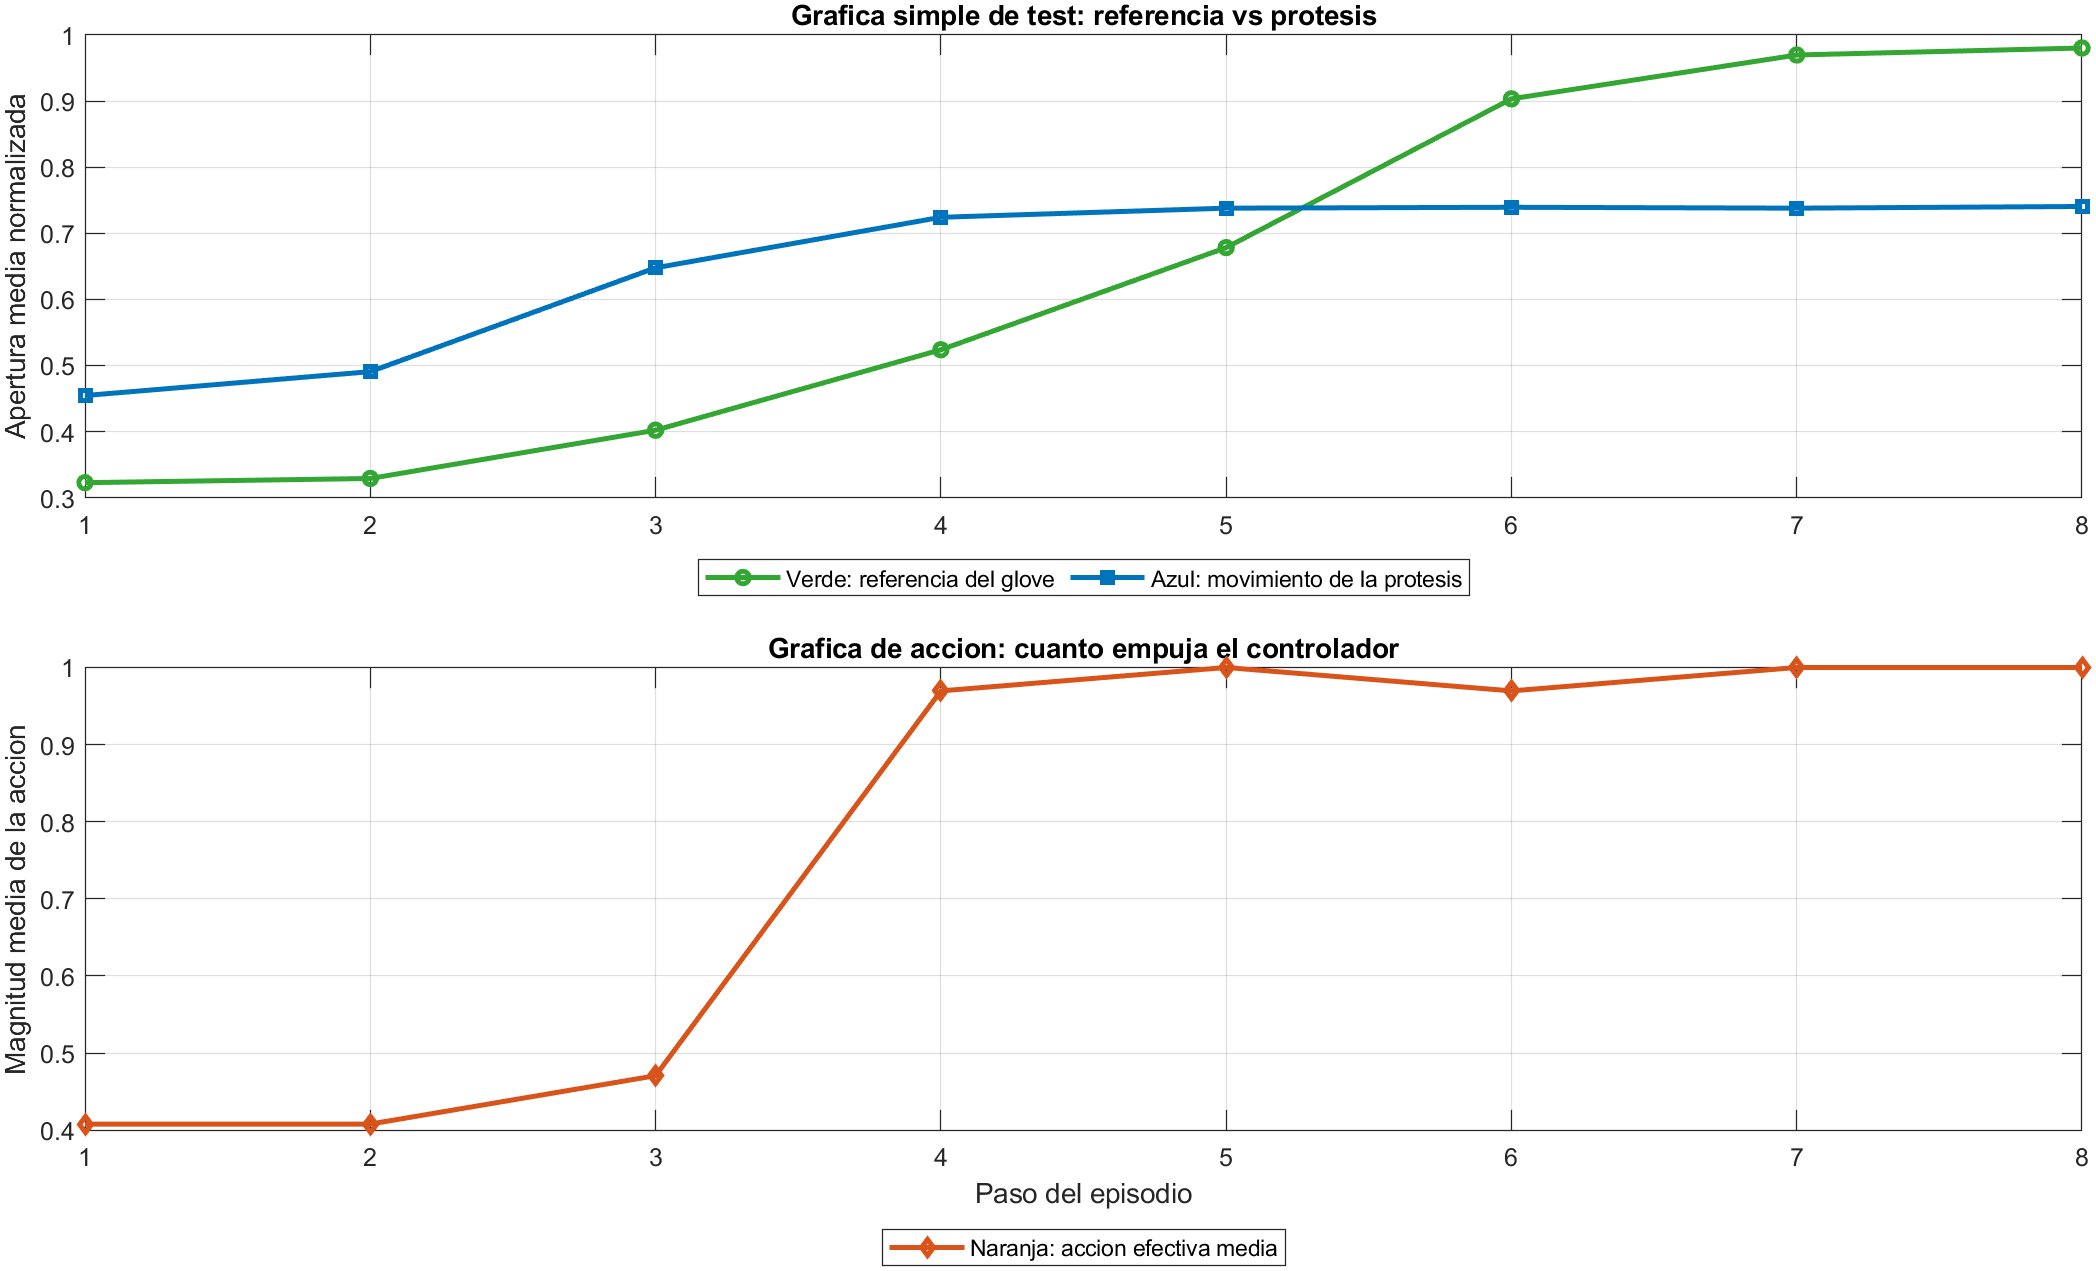
\includegraphics[width=0.96\linewidth]{figures/charla_test_residual_20260326.png}
\caption{Grafica simple de test. Arriba se ve si la protesis sigue a la referencia. Abajo se ve cuanto empuja el controlador.}
\end{figure}

\paragraph{Linea verde.}
Es la referencia del glove. Es el movimiento que la protesis intenta copiar.

\paragraph{Linea azul.}
Es el movimiento real de la protesis. Si va cerca de la verde, el tracking es bueno. Si se queda muy abajo o se separa mucho, el tracking es malo.

\paragraph{Linea naranja.}
Es la magnitud de accion. Sirve para ver cuanta ``fuerza de control'' esta usando el sistema. Si esta siempre muy arriba, la politica es agresiva. Si esta demasiado abajo y la protesis casi no sigue, la politica es timida.

\section{Grafica final de comparacion}

\begin{figure}[H]
\centering
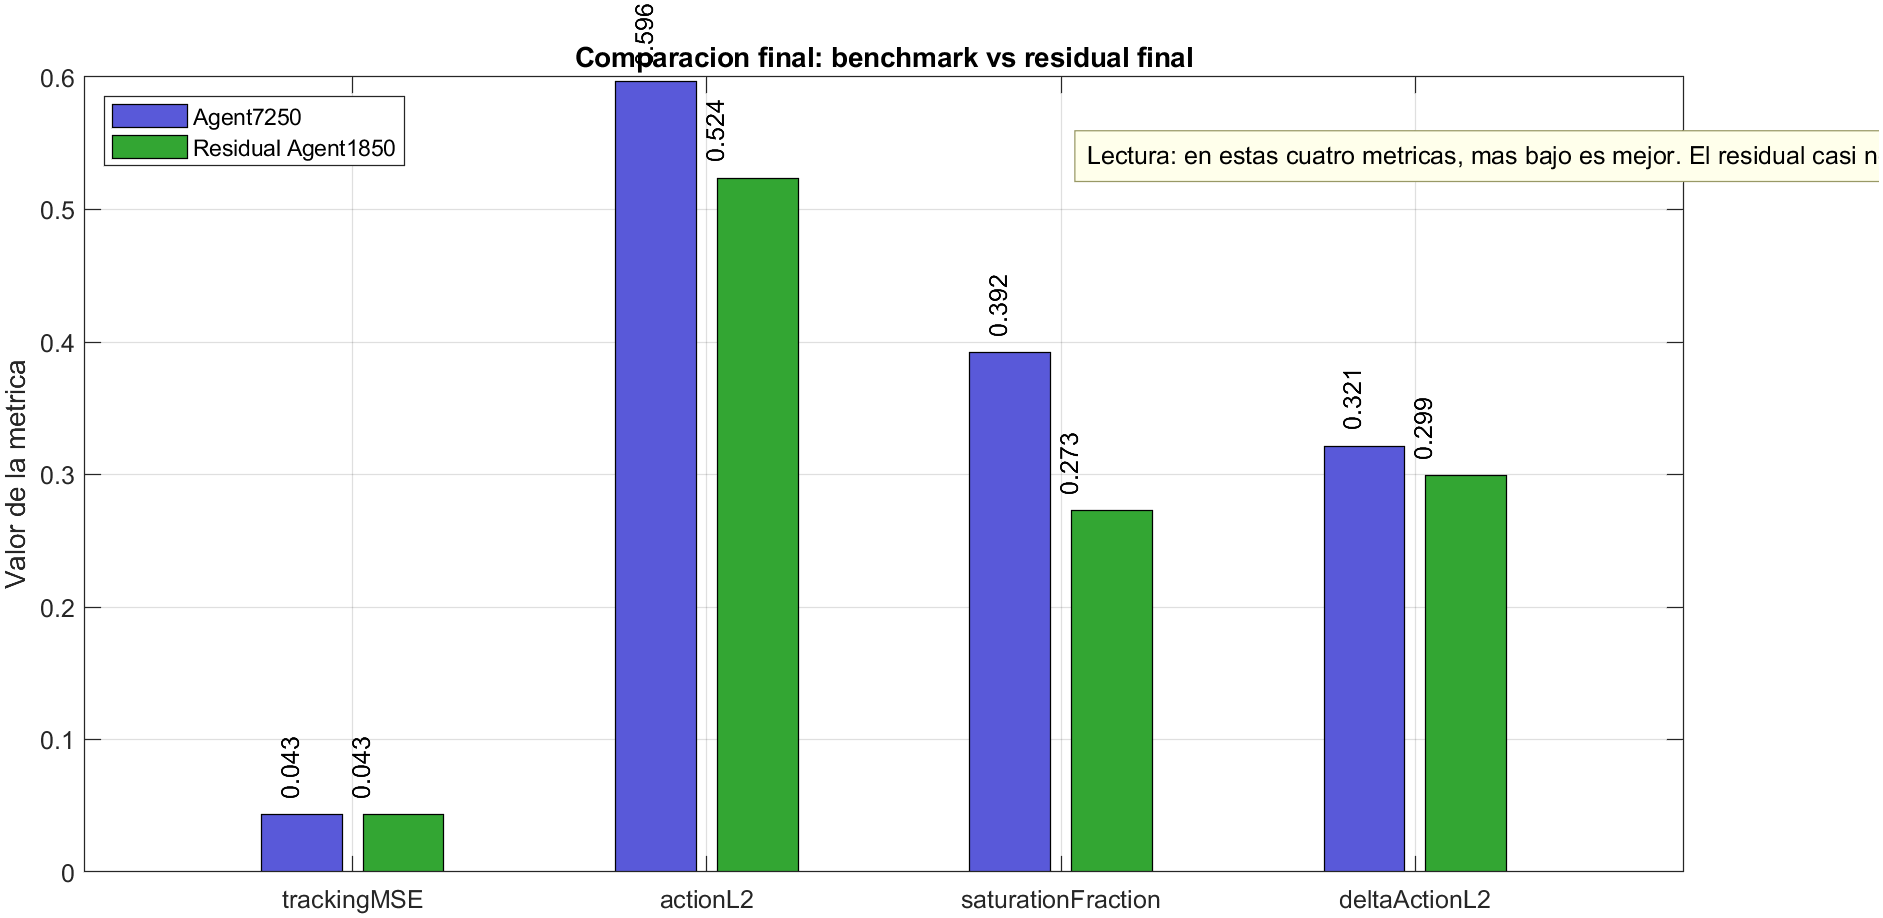
\includegraphics[width=0.94\linewidth]{figures/charla_comparacion_final_20260326.png}
\caption{Comparacion final entre \texttt{Agent7250} y el residual \texttt{Agent1850}.}
\end{figure}

\paragraph{Como leer esta grafica.}
Aqui las cuatro metricas se leen igual: mas bajo es mejor.
\begin{itemize}[leftmargin=1.5em]
\item \textbf{trackingMSE}: error de seguimiento;
\item \textbf{actionL2}: cuanto esfuerzo total usa la accion;
\item \textbf{saturationFraction}: cuanto tiempo se pega al borde;
\item \textbf{deltaActionL2}: que tan bruscos son los cambios.
\end{itemize}

\paragraph{Que cuenta esta grafica.}
El residual final empeora un poco el \texttt{trackingMSE}, pero mejora de forma clara el esfuerzo, la saturacion y la brusquedad. Esa es justamente la idea de una mejora de compromiso.

\section{Que fue el barrido de alpha}

Despues del piloto residual se probaron varios valores de \(\alpha_{\mathrm{res}}\):
\begin{itemize}[leftmargin=1.5em]
\item barrido corto: \(0.10, 0.20, 0.30\);
\item refinamiento fino: \(0.18, 0.20, 0.22, 0.25\).
\end{itemize}

La conclusion fue sencilla:
\begin{itemize}[leftmargin=1.5em]
\item \(0.10\) corregia poco;
\item \(0.30\) corregia demasiado;
\item \(0.20\) quedo en el mejor punto intermedio;
\item el refinamiento fino confirmo que \(0.20\) seguia siendo la mejor opcion.
\end{itemize}

\section{Que significa que el residual haya quedado en ConditionB}

No significa ``gana en todo''. Significa algo mas realista y mas util:
\begin{itemize}[leftmargin=1.5em]
\item no empeora tracking de forma grave;
\item baja saturacion de forma clara;
\item baja esfuerzo total de forma clara.
\end{itemize}

En este proyecto eso fue suficiente para tomar al residual \texttt{Agent1850} como punto final operativo.

\section{Resultado final para contar en la charla}

La forma simple de cerrar la charla puede ser esta:

\begin{quote}
Primero hubo que limpiar el problema. Luego se encontro un benchmark serio, \texttt{Agent7250}. Despues se probaron varias formas de mejorarlo. La que realmente funciono fue no destruir la politica buena, sino corregirla un poco con una politica residual. Asi aparecio \texttt{Agent1850}, que mantiene casi el mismo tracking pero con menos agresividad.
\end{quote}

\section{Fuentes de apoyo}

Para esta charla conviene citar solo la idea principal de cada fuente:
\begin{itemize}[leftmargin=1.5em]
\item el articulo base del proyecto \citep{fuertes2026continuous};
\item el paper original de TD3 \citep{fujimoto2018td3};
\item la revision sobre control mioelectrico \citep{chen2023review};
\item la idea de politica residual \citep{silver2018residual,schaff2020shared,resfit2025};
\item la documentacion de MathWorks para actores continuos y TD3 \citep{mathworks_td3_agent,mathworks_td3_options,mathworks_continuous_actor}.
\end{itemize}

\bibliographystyle{unsrt}
\bibliography{references}

\end{document}
